\documentclass[tikz,border=0mm]{standalone}
\usepackage{tikz}
\usepackage{physics}
\usetikzlibrary{backgrounds,angles,quotes,calc,fit,positioning,decorations.pathreplacing,calligraphy}
\definecolor{navy}{RGB}{30,60,120}

\begin{document}

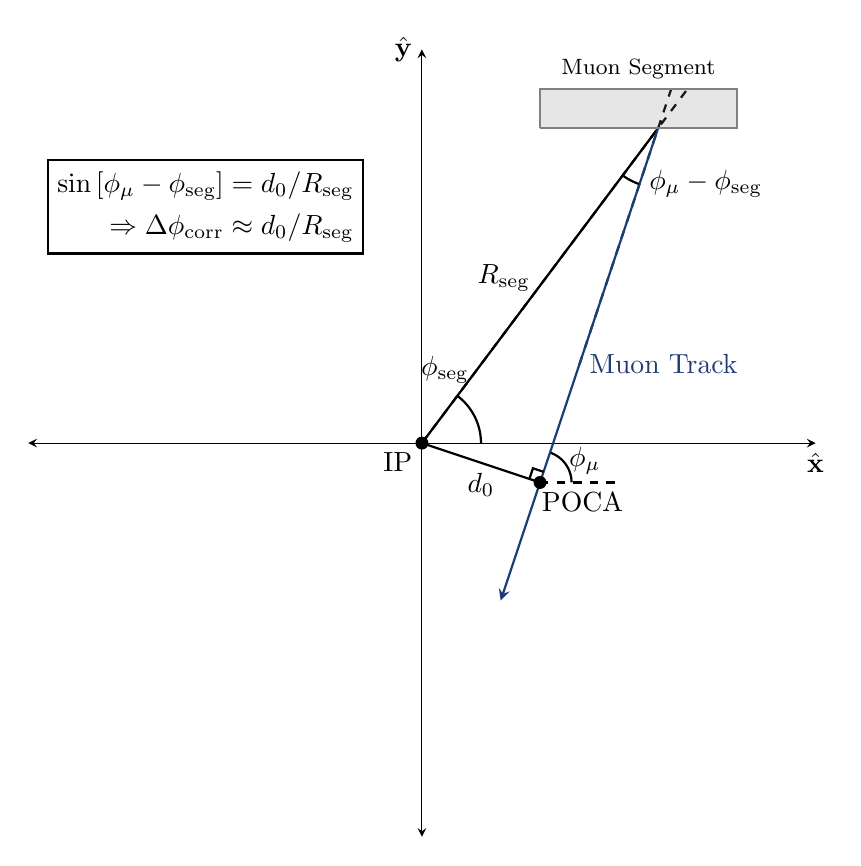
\begin{tikzpicture}
    \draw[thick,dashed,domain=2:3.2] plot({\x},{3*\x-5}) (0,0) -- (3.375,4.5); 
    \draw[stealth-stealth] (-5,0) -- (5,0) node[below]{$\hat{\vb{x}}$};
    \draw[stealth-stealth] (0,-5) -- (0,5) node[left]{$\hat{\vb{y}}$};
    \draw[thick,dashed] (1.5,-0.5) -- (2.5,-0.5);
    \draw[thick] (0,0) -- (3,4) node[left,pos=0.5,yshift=0.1cm]{$R_\text{seg}$};
    \draw[thick,navy,-stealth] (3,4) -- (1,-2) node[right,pos=0.5]{Muon Track};
    \draw[black,fill=black] (0,0) circle (0.075) node[below left]{IP} (1.5,-0.5) circle (0.075) node[below right,xshift=-0.1cm]{POCA};
    \draw[gray,thick,fill opacity=0.2,fill=gray] (1.5,4) -- (4,4) -- (4,4.5) -- (1.5,4.5) -- (1.5,4);
    \draw[black] (2.75,4.5) node[above]{\footnotesize{Muon Segment}};
    \draw[domain=0:54,thick] plot({0.75*cos(\x)},{0.75*sin(\x)}) node[xshift=-0.15cm,yshift=0.325cm]{$\phi_{\text{seg}}$};
    \draw[domain=0:70,thick] plot({1.5+0.4*cos(\x)},{-0.5+0.4*sin(\x)}) node[right,xshift=0.1cm,yshift=-0.1cm]{$\phi_{\mu}$};
    \draw[domain=234:251,thick] plot({3+0.75*cos(\x)},{4+0.75*sin(\x)}) node[right]{$\phi_{\mu}-\phi_{\text{seg}}$};
    \draw[thick] (0,0) -- (1.5,-0.5) node[below,pos=0.5]{$d_0$};
    \draw[thick] (1.365,-0.455) -- (1.41,-0.32) -- (1.545,-0.365);
    \draw (-2.75,3) node[rectangle,draw=black,thick]{
    $\begin{aligned}
    \sin\qty[\phi_{\mu}-\phi_{\text{seg}}]=&\; d_0/R_\text{seg}\\
    \Rightarrow \Delta\phi_{\text{corr}}\approx&\; d_0/R_\text{seg}\end{aligned}$};
\end{tikzpicture}

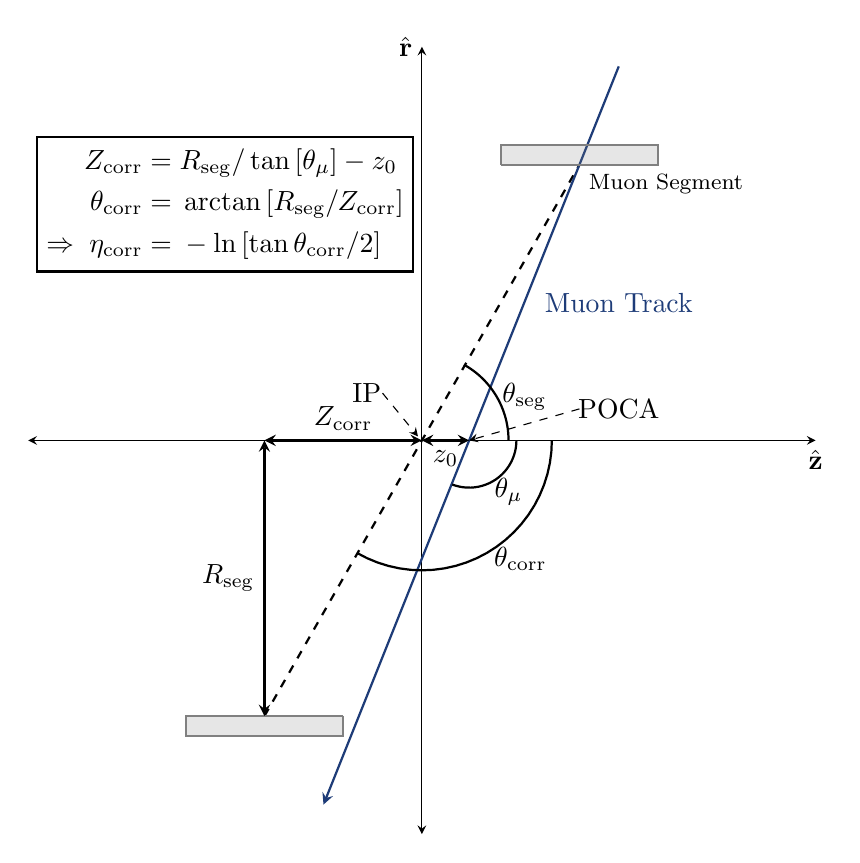
\begin{tikzpicture}
    \draw[stealth-stealth] (-5,0) -- (5,0) node[below]{$\hat{\vb{z}}$};
    \draw[stealth-stealth] (0,-5) -- (0,5) node[left]{$\hat{\vb{r}}$};
    \draw[domain=-2:2,thick,dashed] plot({\x},{1.75*\x});
    \draw[domain=-1.25:2.5,thick,stealth-,navy] plot({\x},{2.5*\x-1.5}) node[xshift=0cm,yshift=-3cm]{Muon Track};
    \draw[gray,thick,fill opacity=0.2,fill=gray] (1,3.5) -- (3,3.5) -- (3,3.75) -- (1,3.75) -- (1,3.5);
    \draw[gray,thick,fill opacity=0.2,fill=gray] (-1,-3.5) -- (-3,-3.5) -- (-3,-3.75) -- (-1,-3.75) -- (-1,-3.5);
    \draw[black] (2,3.75) node[yshift=-0.5cm,xshift=1.1cm]{\footnotesize{Muon Segment}};
    \draw[stealth-stealth,thick,black] (0,0) -- (-2,0) node[above,pos=0.5]{$Z_{\text{corr}}$};
    \draw[stealth-stealth,thick,black] (0,0) -- (0.6,0) node[below,xshift=-0.3cm]{$z_0$};
    \draw[stealth-stealth,thick,black] (-2,0) -- (-2,-3.5) node[left,pos=0.5]{$R_{\text{seg}}$};
    \draw[domain=0:61,thick] plot({1.1*cos(\x)},{1.1*sin(\x)}) (1.3,0.55) node[]{$\theta_{\text{seg}}$};
    \draw[domain=249:360,thick] plot({0.6+0.6*cos(\x)},{0.6*sin(\x)}) (1.1,-0.65) node[]{$\theta_{\mu}$};
    \draw[domain=240:360,thick] plot({1.65*cos(\x)},{1.65*sin(\x)}) (1.25,-1.5) node[]{$\theta_{\text{corr}}$};
    \draw[dashed,thin,-stealth] (2,0.4) -- (0.6,0) node[pos=0.0,xshift=0.5cm]{POCA};
    \draw[dashed,thin,-stealth] (-0.5,0.6) -- (-0.05,0.05) node[pos=0.0,xshift=-0.2cm]{IP};
    \node[rectangle,draw=black,thick] at (-2.5,3) {$
    \begin{aligned}
    Z_{\text{corr}}=&\;R_{\text{seg}}/\tan\qty[\theta_{\mu}]-z_0\\    \theta_{\text{corr}}=&\;\arctan\qty[R_{\text{seg}}/Z_{\text{corr}}]\\\Rightarrow \;\eta_\text{corr}=&\;-\ln\qty[\tan{\theta_\text{corr} }/{2}]
    \end{aligned}$
    };
\end{tikzpicture}

\end{document}